\documentclass{article}
\usepackage[margin=1.0in]{geometry}
\usepackage{authblk} %package for blocking authors, followed by blocking affiliation
\usepackage{url}
\usepackage{ulem} % when using ulem package, must change \emph to \it for italics.
\usepackage{hyperref}
\usepackage{array}
\usepackage{amssymb,amsmath,tabu}
\usepackage{hyperref}
\setlength\parindent{0pt}
\usepackage[english]{babel}
\usepackage{graphicx}
\usepackage{enumitem}

\begin{document}
\title{Homework 1\\ SOCI 303: Statistics for the Social Sciences (Spring 2017) \\ {\large{10 points}}}
\author[*]{}
\date{}
\maketitle



\section*{Overview:}
In this assignment, you'll be completing 10 problems from the ``Chapter Exercises'' section of Chapters 1 through 5. This homework assignment may be typed up or hand written or a combination of both.

\subsection*{Chapter 1 Problems}
\begin{itemize}
\item 3 (a, b, c, d, e, f, g, h) 
	\begin{enumerate}[label=(\alph*)]
	\item Interval-ratio
	\item Nominal
	\item Interval-ratio
	\item Ordinal
	\item Nominal
	\item Interval-ratio
	\item Interval-ratio
	\item Nominal 	
	\end{enumerate}
\item 6 (a, b, d, e) 
	\begin{enumerate}[label=(\alph*)]
	\item Unemployment records could be used to determine the actual number of unemployed; a descriptive statistic based upon the population. 
	\item A survey is taken to estimate student opinions about the quality of food; inferential statistic. \addtocounter{enumi}{1} %enumi controls \items at first level, enumii at second, enumiii at third, enumiv at fourth. 1 adds 1 `step' to the following item... essentially skips one step/number/letter, 2 skips two.
	\item The ratings will be gathered from a survey, so this is inferential.
	\item A university should be able to report GPA by major, so this is a descriptive statistic based upon the population. 
	\end{enumerate}
\end{itemize}

\subsection*{Chapter 2 Problems}
\begin{itemize}
\item 1 (a, b) 
	\begin{enumerate}[label=(\alph*)]
	\item Race is a nominal variable. Class is an ordinal variable, since the categories can be ordered from lower to higher status. 
	\item \begin{tabular}{ | l | c | }
	\hline
    	Race & Frequency ($f$)  \\ \hline
    	White & 17  \\ \hline
	Nonwhite & 13  \\ \hline
    	Total & 30  \\ 
	\hline
	\end{tabular}
	\end{enumerate}
\item 6 (a, b) 
	\begin{enumerate}[label=(\alph*)]
	\item \begin{tabular}{ | l | c | c | c | c | }
	\hline
	Email hours per week & Frequency & Cf & \% & C\%  \\ \hline
	0 & 19 & 19 & 19 & 19 \\ \hline
	1 & 20 & 39 & 20 & 39 \\ \hline
	2 & 13 & 52 & 13 & 52 \\ \hline
	3 & 5 & 57 & 5 & 57 \\ \hline
	4 & 2 & 59 & 2 & 59 \\ \hline
	5 & 6 & 65 & 6 & 65 \\ \hline
	6 & 5 & 70 & 5 & 70 \\ \hline
	7 & 2 & 72 & 2 & 72 \\ \hline
	8 & 3 & 75 & 3 & 75 \\ \hline
	9 & 1 & 76 & 1 & 76 \\ \hline
	10 or more  & 23 & 99 & 23 & 99 \\ \hline
	Total  & 99 &  &  99\% & \\
	\hline 
	\end{tabular} \\
	\item .575 (57/99) spent 3 hours or less on email per week.
	\end{enumerate}
\end{itemize}

\subsection*{Chapter 3 Problems}
\begin{itemize}
\item 4
	\begin{itemize}
	\item 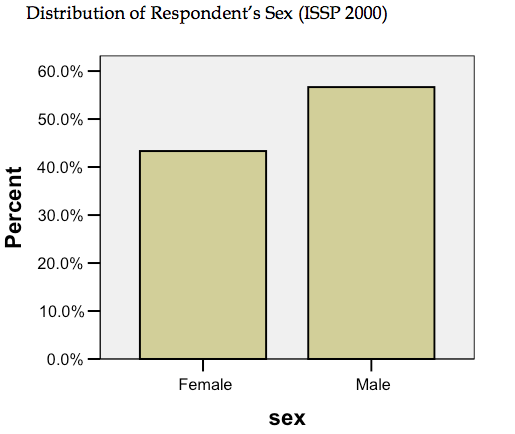
\includegraphics[scale=.5]{/Users/burrelvannjr/Dropbox/stats_csuf/hw/hw1/sex_graph.png} \\ \\ 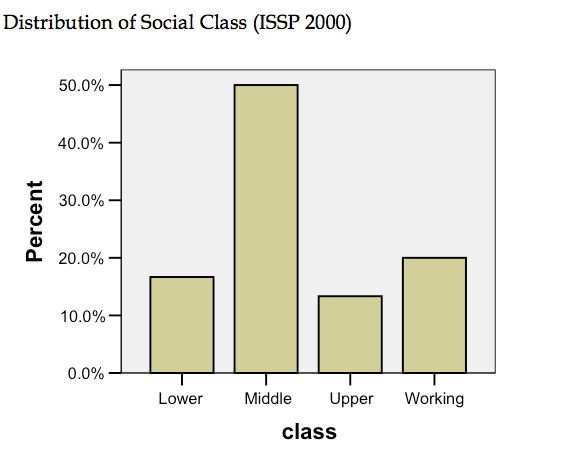
\includegraphics[scale=.5]{/Users/burrelvannjr/Dropbox/stats_csuf/hw/hw1/class_graph.png}
	\end{itemize}
\end{itemize}

\subsection*{Chapter 4 Problems}
\begin{itemize}
\item 1 (a, b, c, d) 
	\begin{enumerate}[label=(\alph*)]
	\item The mode is ``Exciting.''
	\item $\frac{N + 1}{2} = \frac{974 + 1}{2} = $487.5th case. Find where the 487th and 488th cases fall. Both of these cases correspond to the category ``Routine,'' which is the median.
	\item The mode is simply the category with the highest frequency (or percentage) in the distribution. The median divides the distribution into two equal parts so that half the cases are below it and half above it.
	\item Because this variable is an ordinal-level variable.
	\end{enumerate}
\item 7 
	\begin{enumerate}[label=(\alph*)]
	\item \begin{tabular}{ | c | c | c | }
	\hline
    	Household Size & Frequency & Frequency x Y ($f$Y) \\ \hline
	1 & 381 & 381 \\ \hline
	2 & 526 & 1,052 \\ \hline
	3 & 227 & 681 \\ \hline
	4 & 200 & 800 \\ \hline
	5 & 96 & 480 \\ \hline
	6 & 42 & 252 \\ \hline
	7 & 19 & 133 \\ \hline
	8 & 5 & 40 \\ \hline
	9 & 2 & 18 \\ \hline
	10 & 2 & 20 \\ \hline
	Total & $N$ = 1,500 & $\Sigma f$Y = 3,857 \\ 
	\hline
	\end{tabular}
	\end{enumerate}
	$\bar{Y}$ = $\frac{\Sigma fY}{N}$ = $\frac{3857}{1500}$ = $2.5713$ \\
\item 9 (a, b) 
	\begin{enumerate}[label=(\alph*)]
	\item There appear to be a few outliers (i.e., extremely high values); this leads us to believe that the distribution is skewed in the positive direction. \\ 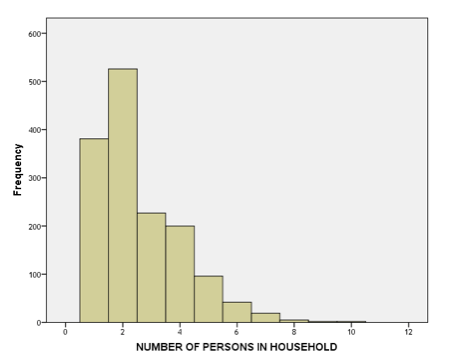
\includegraphics[scale=.5]{/Users/burrelvannjr/Dropbox/stats_csuf/hw/hw1/skew_graph.png}
	\item The median can be found two ways: by using either the frequencies column or the cumulative percentages. The data are in frequencies; we?ll use those to solve the median. Since the median (2) is less than the mean (2.57), we can conclude that the distribution is skewed in a positive direction. Our answer to question 9a is further supported.
	\end{enumerate}
\end{itemize}

\subsection*{Chapter 5 Problems}
\begin{itemize}
\item 5 (a, b, c) 
	\begin{enumerate}[label=(\alph*)]
	\item The range of projected increase in the elderly population for the western states is 36.2\%. The range of percent increase for the Midwestern states is 9.8\%. The western states have a much larger range. 
	\item The IQR for the western states is 17.3\%. The IQR for the Midwestern states is 3.7\%. Again, the value for the western states is greater.
	\item There is great variability in the projected increase in the elderly population in western states, resulting from large increases in Nevada, Arizona, Wyoming, and Alaska, as measured by either the range or the IQR.
	\end{enumerate}
\item 8 (a, b) 
	\begin{enumerate}[label=(\alph*)]
	\item For those diagnosed with cancer: \\
	\begin{center}
	Variance = $\frac{\Sigma (Y-\bar{Y})^2}{N - 1}$ = $\frac{3059.14}{187 - 1}$ = 16.45 \\ \vskip2ex
	$SD$ = $S_Y$ = $\sqrt{S^2_{Y}}$ = $\sqrt{\frac{\Sigma (Y-\bar{Y})^2}{N - 1}}$ = $\sqrt{\frac{3059.14}{187 - 1}}$ = $\sqrt{16.45}$ = 4.06 \\ \vskip2ex
	\end{center}
	For those NOT diagnosed with cancer: \\
	\begin{center}
	Variance = $\frac{\Sigma (Y-\bar{Y})^2}{N - 1}$ = $\frac{25180.20}{1200 - 1}$ = 21 \\ \vskip2ex
	$SD$ = $S_Y$ = $\sqrt{S^2_{Y}}$ = $\sqrt{\frac{\Sigma (Y-\bar{Y})^2}{N - 1}}$ = $\sqrt{\frac{25180.20}{1200 - 1}}$ = $\sqrt{21}$ = 4.58 \\ \vskip2ex
	\end{center}
	\item Although there is a slightly more variability in psychological distress score among those not diagnosed with cancer than those diagnosed with cancer, the standard deviations of the two groups are very close (4.58 vs. 4.06). An interesting finding is that the respondents diagnosed with cancer are not only slightly less diverse in terms of the distress level, but their average psychological distress score is also less than those not diagnosed with cancer (3.9 vs. 4.87).
	\end{enumerate}
\end{itemize}


\end{document}











